\chapter{Energetics of Locomotion}
\label{sec:EnergeticsOfLocomotion}
\index{energetics}

In this book, the description of locomotion has been grounded in understanding the relevant dynamics through energy. Chapter \ref{sec:Introduction} introduced the cost of transport $COT$ as a metric for locomotion. Chapter \ref{sec:PropertiesOfMotorsAndMuscles} describes the peak power that muscles can produce, and introduces the metric of \textit{metabolic cost}. The models developed in chapter \ref{sec:ModelingLeggedLocomotion} include discussions of metabolic cost and energy loss from collisions.

Energy is such an important aspect of locomtion because it seems that locomotives may move in such a way as to minimize the metabolic cost of locomotion. Likewise, the metabolic cost can be minimized for the models of locomotion presented in this text. If the metabolic cost of locomtion is available for a given dynamics model of locomotion, then it may be possible to determine the parameters of the model that minimize that cost. These ideas are explored in chapter \ref{sec:OptimizationInLocomotion}. This chapter serves to bridge the topics that have been explored already to the ideas of energy optimization by providing a more thorough background in energy and muscle work.

\section{Power for Mechanical Systems} %(notes page 39, 43-49)
\label{sec:PowerforMechancialSystems}

This section contains a review of some fundamental ideas in classical dynamics, and moves onto some thermodynamics and a description of muscles that extends beyond what was presented in Chapter \ref{sec:PropertiesOfMotorsAndMuscles}.

The systems considered in introductory dynamics courses often do not require one to consider internal forces. This is fine, because it is only the external forces and torques that must be present in equations of momentum balance. After all, internal forces do not appear in free body diagrams.  Internal forces are usually more relevant in a statics course, or for analyzing failure of a system; they are not required for determining rigid body motion with momentum balance.  However, internal forces are relevant when using energy and power to describe motion.  Accordingly, a locomotive's motion depends on both internal forces and external forces. The free body diagram of a car only includes external forces, such as gravity, normal forces, and friction. The internal forces do not appear in a free body diagram of the entire car, but would appear in a free body diagram of just the engine, or of just the transmission (figure \ref{fig:CarForces}).

% FIGURE
\begin{figure}[h]		% h="here" t="top" b="bottom" p="separate page"
\begin{centering}
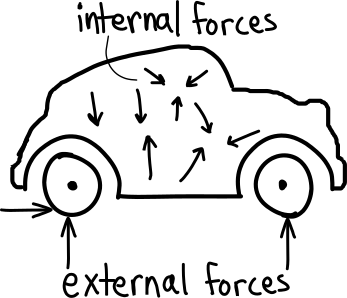
\includegraphics[width=0.3\textwidth]{Figures/CarForces}\par
\end{centering}
\caption[Diagram: Forces in and on a car]{Forces in and on a car. During typical operation, a car has both internal forces and external forces acting upon it. The internal forces may arise from the transmission or the passengers, while the external forces consists of gravity, ground reaction, and friction.}
\label{fig:CarForces}
\end{figure}
%

Humans, animals and robots are like cars in that they are not propelled solely by external forces (such is the case with point masses). What implications does this have for energy, and more intuitively, power? It is enlightening to develop equations for power with a distinction between internal and external forces. The instantaneous power required to force a particle that is traveling at a velocity $\vv$ is

\begin{align}
\vF_{tot} \cdot \vv  &=  m\va \cdot \vv = \frac{d}{dt} \left(\frac{m v^2}{2}\right) \\
 P &= \KEdot
\end{align}

where the chain rule of differentiation has been employed, $d(v^{2})/dt = 2v(dv/dt)$. This provides the logical work-energy theorem result for a particle, that $P = \dot{\KE}$. Of course in this case the total force is also the total external force, since a single particle cannot have any internal forces.

The power required to move a collection of particles, or a system of particles and rigid bodies, is

\begin{align}
 \sum_{i} \vF_{i} \cdot \vv_{i}  &=  \sum_{i} \frac{d}{dt}\left(\frac{m_{i} v_{i}^{2}}{2}\right) = \sum_{i} \KEdot_{i}\\
P^{tot} &= \KEdot
\label{eq:PowerCollectionOfParticles}
\end{align}

where $\vF_{i}$ is the total force on particle $i$ whose velocity is $\vv_{i}$, and $\KEdot$ is the time rate of change of the system's total kinetic energy. Equation \ref{eq:PowerCollectionOfParticles} can be used to describe the power developed with a system as simple as a two-particle system, or as complicated as a car. In the latter case, the system is comprised mostly of rigid bodies, in which case the forces and velocities are of the centers of mass of the rigid bodies.

As we mentioned, it is important to make a distinction between internal and external forces. Consider a collection of particles (no rigid bodies). The total force on particle $i$ can be split up as $\vF_{i} = \vF_{i}^{int} + \vF_{i}^{ext}$. If we make this distinction, the power can be written as the sum of an internal power and an external power.

\begin{align}
P^{tot} &= \sum_{i} (\vF_{i}^{int} + \vF_{i}^{ext}) \cdot \vv_{i} = P^{int} + P^{ext}\\
P^{int} &= \sum_{i} \vF_{i}^{int} \cdot \vv_{i} \\
P^{ext} &= \sum_{i} \vF_{i}^{ext} \cdot \vv_{i}
\end{align}

The power-\.{energy} relationship is then

\begin{align}
P_{tot} &=  \KEdot\\
P^{int} + P^{ext} &= \KEdot_{/G} + \KEdot_{G}
\label{eq:PowerInternalExternal}
\end{align}

where $\KEdot_{/G}$ is the time derivative of the sum of the kinetic energy of each particle with respect to the center of mass of the system, and $\KEdot_{G}$ is the time derivative of the kinetic energy of the center of mass of the system. Accordingly, these last two terms are

\begin{align}
\KEdot_{/G} &= \frac{d}{dt} \sum_{i} \frac{m_i}{2}(v_{i} - v_{G})^{2} = \frac{d}{dt} \sum_{i} \frac{m_i}{2} v_{i/G}^{2} \\
\KEdot_{G} &= m_{T} \frac{d}{dt} v_{G}^{2}
\end{align}

where $v_{G}$ is the speed of the center of mass of the system, and $m_{T} = \sum m_i$ is the total mass of the system. These two equations come from Konig's theorem, equation \ref{eq:Konig}, which was derived in \ref{sec:EquationsOfMotion}. We arrived at equation \ref{eq:PowerInternalExternal} by working with power rather than work because the math for power is simpler. For a formulation that starts with work instead, refer to the classical dynamics text by Greenwood \cite{greenwood}.

Equation \ref{eq:PowerInternalExternal} describes power through a sum of internal forces and external forces, and describes the time rate of change of kinetic energy as a sum of a ``relative'' kinetic energy, and a center of mass kinetic energy. It may seem that these terms correspond to each other; that the internal forces cause an internal power equivalent to $\KEdot_{/G}$ and that the external forces cause an external power equivalent to $\KEdot_{G}$. For example, if a car is in neutral and the driver depresses the accelerator, then the car has internal forces that contribute to an internal power that \textit{is} equivalent to $\KEdot_{/G}$ since the engine does turn. There is no external power since the external forces ground reaction act at stationary points and $\KEdot_{G} = m_{T}(0)^2/2 = 0$. The proposed correspondence holds.

However, this correspondence is incorrect in general. Consider the car in figure \ref{fig:CarForces} once again. A free body diagram of this car illustrates that if the car is accelerating, its acceleration is a result of the horizontal external force acting at the bottom of its wheels. Additionally, $\KEdot_{G}$ is increasing since it is a function of $v_{G}$. While this external force is necessary to give rise to $\KEdot_{G}$, this force does not create the power that contributes to $\KEdot_{G}$. The velocity of a wheel at the point at which the horizontal external friction force is instantaneously zero from the no-slip condition. Thus, this external force does not produce any power. Instead, the relation between external force and $\KEdot_{G}$ is developed by first noting that

\begin{equation}
\KEdot_{G} = \frac{d}{dt} \KE_{G} = m_{T}  \frac{d}{dt} (\vv_{G} \cdot \vv_{G}) = m_{T} \va_{G} \cdot \vv_{G}
\end{equation}

and then by dotting Newton's second law with $\vv_{G}$

\begin{align}
( \vF^{ext} &= m_{T} \va_{G} ) \cdot \vv_{G} \\
\vF^{ext} \cdot \vv_{G} &= \KEdot_{G} \label{eq:CarExternalForce}
\end{align}

The left hand side of equation \ref{eq:CarExternalForce} is \emph{not} external power (the term is revisited later), but nonetheless the external force can be seen to relate to the center of mass kinetic energy of the car. The internal forces that generate power that contribute to $\KEdot_{G}$ are in the engine, the transmission, and so on. While it is possible to develop physically meaningful conceptions of mass, acceleration, force, and kinetic energy, the left hand side of equation \label{eq:CarExternalForce} has no perceptible conceptual or physical meaning.

We elucidate this distinction by using one of the simplest systems of particles possible, as described in figure \ref{fig:ParticleExplosion}. Two masses are attached to each other by a spring with spring constant $k$, and the right mass is fixed to a wall. The system is excited, and the left mass oscillates. The center of mass of the two particle system is located at the midpoint between the masses. There is an external reaction force from the surface on the right particle, $F_{ext}$ that enforces the fixed constraint on the right mass.

% FIGURE
\begin{figure}[h]		% h="here" t="top" b="bottom" p="separate page"
\begin{centering}
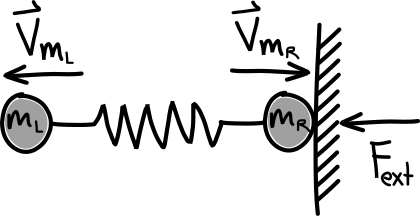
\includegraphics[width=0.4\textwidth]{Figures/ParticleExplosion}\par
\end{centering}
\caption[Diagram: Two Masses on a Spring]{Two masses on a spring. Two masses are attached to each other by a spring with spring constant $k$, and the right mass is fixed to a wall. This simple example can illustrate how  internal and external power contribute to the kinetic energy of a system of particles. The external reaction force acts at a stationary mass, and thus does not produce any power. It is rather the internal power generated by the spring force that gives rise to the kinetic energy of both the left mass and the system of particles.}
\label{fig:ParticleExplosion}
\end{figure}
%

In this example, it is clear that $\KEdot_{G}$ is nonzero, since the center of mass has motion, but this motion arises from the power developed by the internal spring force $k\Delta x$, not from the external reaction force $F_{ext}$. The external reaction force acts at a stationary point, and thus does not develop any power. In the limit as $m_L/m_R \rightarrow \infty$, the system becomes a single oscillating mass, and the internal work becomes equivalent to the center of mass kinetic energy.

Thus, the relation between internal power, external power, ``relative'' kinetic energy and center of mass kinetic energy is more elusive than it may seem at first.

\subsection*{Power in Biomechanics}
\label{sec:Power in Biomechanics}
\index{external power}

In biomechanics, the terms ``internal power'' and ``external power'' do not
refer to the terms $P^{int}$ and $P^{ext}$ as they have been defined in this
text. We can clarify this difference for systems of point masses (no rigid
bodies). The biomechanics internal power $P_{bio}^{int}$ and external power
$P_{bio}^{ext}$ are defined by

\begin{align}
P_{bio}^{int} &= \sum_{i} F_{i} \cdot \vv_{i/G} \\
P_{bio}^{ext} &= \sum_{i} F_{i}^{ext} \cdot \vv_{G} = \vv_{G} \cdot \sum_{i} F_{i}^{ext}
P^{tot} &= P_{bio}^{int} + _{bio}^{ext} \\
\end{align}

The biomechanics internal power is the sum across particles of the \emph{total}
force on each particle multiplied with its velocity \emph{relative to the
center of mass}. The biomechanics external power is the sum across particles of
the total external force on each particle multiplied with the velocity of the
entire system's center of mass. This is equivalent to treating the system as a
single point mass with velocity $v_{G}$ and with a total external force
$F^{ext} = \sum F_{i}^{ext}$ acting upon it.

The biomechanics power terms have the nice feature that

\begin{align}
P_{bio}^{int} &= \KEdot_{/G} \label{eq:PbioInt}  \\
P_{bio}^{ext} &= \KEdot_{G}  \label{eq:PbioExt}
\end{align}

However, this is the extent of the usefulness of the biomechanics usage of internal power and external power. Additionally, 

\begin{itemize}
\item The definition of power requires that in the term $\vF \cdot \vv$, the
    force $\vF$ acts at the point which has velocity $\vv$. This is not true
    for $P_{bio}^{ext}$, since external forces do not necessarily act at the
    center of mass of a system (the system may not even have physical material
    at the center of mass).
\item The biomechanics power definitions cannot be related to the power
    generated by actuators or muscles.
\item The mechanics power definitions have the benefit that to evaluate power,
    the velocities of points at which no force is applied do not need to be
    known. If the force at a point $F_{i}$ is zero, then $F_{i}\cdot\vv_{i} = \mathbf{0} \cdot \vv_{i} =
    0$.
\item $P_{bio}^{int}$ is never useful and never provides any insights, and also counterintuitively depends on external forces.
\item $P_{bio}^{ext}$ is only useful for particle models.
\end{itemize}

In the biomechanics literature, the phrases ``internal power'' and ``external
power'' are often confused as referring to the terms $P^{int}$ and $P^{ext}$,
while the phrases actually refer to the $P_{bio}^{int}$ and $P_{bio}^{ext}$.
Keep in mind that the discussion here focuses on particle systems, and not
systems of rigid bodies.

\subsection*{Rigid object systems}

A locomotive can be approximated as a system of linked rigid bodies. Potentially, a locomotive is modeled better as a system of linked rigid bodies than as a collection of point masses, especially if the aim is to understand how muscles affect the motion of the locomotive. The time rate of change of the total kinetic energy of a locomotive $\KEdot$ can be expressed in terms of the forces and moments acting on the rigid bodies that compose a locomotive in a way that is slightly more detailed than equation \ref{eq:PowerInternalExternal}.  Again, the locomotive can have both internal and external forces. Starting from equation \ref{eq:PowerInternalExternal} and noting that $\vv_i = \vv_{G} + \vv_{i/G}$ and $\vv_{i/G} = \vomega_{G} \times \vec{\mathbf{r}}_{i/G}$, the power-\.{energy} relation is

\begin{align}
\KEdot &= P^{tot} \notag \\
 &= \sum_{i} (\vF_{i}^{int} + \vF_{i}^{ext} ) \cdot ( \vv_{G} + \vomega_{G} \times \vec{\mathbf{r}}_{i/G})
\end{align}

The right hand side can be expanded, and one of the resulting terms is

\begin{equation}
\sum \vF_{i}^{int} \cdot (\vomega_{G} \times \vec{\mathbf{r}}_{i/G}) \notag
\end{equation}

Using vector properties, this term can be rewritten as

\begin{equation}
\vomega \cdot \sum \vec{\mathbf{r}}_{i/G} \times \vF_{i}^{int} \notag
\end{equation}

This term vanishes, since according to Newton's second law, each internal force on a link also has an equal and opposite force acting on some other link. Through other simplifications, the power-\.{energy} relation eventually becomes

\begin{equation}
\KEdot = \sum_{i} \vF_{i}^{ext} \cdot \vv_{i} + \sum_{i} \vomega_{G} \times \vM_{i}^{ext}
\end{equation}

where $\vM_{i}^{ext}$ is the total external moment on link $i$. Thus, the energy of a rigid body system only depends on external forces and external moments. This conclusion seems to contradict the earlier statement that indicates that the kinetic energy of the center of mass of the system can recieve contribution from internal forces and internal power. [chris: doesn't it?] Consult any standard advanced dynamics textbook for a more thorough understanding of this derivation.

\section{Thermodynamics of Locomotives}
\label{sec:ThermodynamicsofLocomotives}
\index{thermodynamics}

In the context of internal forces an internal power, it makes sense to apply to the First Law of Thermodynamics to a model of a locomotive. Thermodynamics is particularly useful when trying to perform experiments on locomotives: how can metabolic cost be measured? Answering such a question requires knowledge of the ways that energy flows about a body. Previously, we have only dealt with the total \emph{mechanical} energy. The total energy of a locomotive, which is a closed system, is the sum of its kinetic energy $\KE$ and its internal energy $U$. Potential energy is neglected. The time rate of change of the total energy of a locomotive is

\begin{equation}
\KEdot + \dot{U} = P^{ext} + \dot{Q} + \dot{W}
\label{eq:Thermodynamics1}
\end{equation}

The external power $P^{ext}$ arises from friction, the heat input term $\dot{Q}$ arises from temperature differences, and the work term $\dot{W}$ arises from external work input to the system. Friction and the work term can be neglected, since sliding does not often occur with locomotives and so no power is lost to friction, and no odd external work inputs are considered. The time rate of change of the internal energy of the locomotive is

\begin{equation}
\dot{U} = -P^{int} + [\mbox{heat source}] + \dot{E}_{chem}
\label{eq:Thermodynamics2}
\end{equation}

The power terms are logically separated along the internal-external divide: the internal power is part of the time derivative of the internal energy. The $P^{int}$ term must have a negative sign in front of it to remain consistent with equation \ref{eq:PowerInternalExternal}, but because any energy used to do work inside the system must obtain that energy from the system. In the example of the car, the internal power in the engine related with the force of combustion products against piston heads comes from decreasing the enthalpy of the combustion products. For familiarity, the heat production term is commonly expressed in heat transfer texts as $\dot{q}'''V$, a heat production density multiplied by a volume. This can come from internal friction of body parts, but more likely from the heat produced by the inefficiency of thermodynamic processes. The chemical energy $\dot{E}_{chem}$ is the useful energy that is made available by the processing of chemicals such as ATP or fat. It is this term that is related to the oxygen consumption of animals that is often used to measure the metabolic cost of locomotion.

Combining equations \ref{eq:Thermodynamics1} and \ref{eq:Thermodynamics2}, the assumptions for $P^{ext}$ and $\dot{W}$, and expanding the kinetic energy term provides

\begin{equation}
P^{int} + (\dot{Q} - [\mbox{heat prod}]) - \dot{E}_{chem} = \KEdot_{/G} + \KEdot_{G}
\end{equation}

Typically, $\dot{Q} < 0$ since the body is at a higher temperature than the surrounding atmosphere, and $\dot{E}_{chem} < 0$ so that energy is removed from the internal energy of the body and is made useful as kinetic energy. The heat flow terms have been grouped to provide a net heat flow term for clarity.

\section{Locomotives and Muscle Power}
\label{sec:LocomotivesAndMusclePower}
\index{muscle power}

The general ideas presented so far can now be applied in a more direct fashion to humans and animals. Just as the engine in an automotive gives rise to internal forces and power that ultimately move the automobile, the muscles in an animal give rise to internal power that move the locomotive. The following assumptions and simplifications are made

\begin{itemize}
\item \textbf{Negligible gravity power:} Logically, this text is only concerned with mostly horizontal translation of the locomotion's center of mass. Thus, the force of gravity does not create a substantial external power (the force of gravity is perpendicular to the center of mass's velocity, and so the dot product of the two quantities is small). This would not be true for locomotion down or up a substantial incline.
\item \textbf{Negligible friction power:} Energy is not removed from the system (the locomotive) by either air friction or sliding. Sliding can occur, but only for a frictionless contact.
\item \textbf{Negligible ground deformation:} Energy is not removed from the system as a result of the collisions of limbs with the ground.
\end{itemize}

To a large extent, these assumptions are made so that the $P^{ext}$ term in the thermodynamic energy balance can be neglected. Additionally, internal friction is also neglected. Internal friction can come from frictional joints or from the inelastic compression of non-muscle soft tissue. As a result, the only relevant power source (or sink) in the system is the internal power generated by muscles or by joints in the locomotive. That is,

\begin{equation}
P = P^{int} + \cancel{P^{ext}} = \sum_{i} P_{i}^{joint} + \sum_{j} P_{j}^{musc}
\end{equation}

A joint, such as an elbow, can be analyzed by first developing a free body diagram of the joint, as in figure \ref{fig:ElbowFBD}.

%
% FIGURE
\begin{figure}[h]		% h="here" t="top" b="bottom" p="separate page"
\begin{centering}
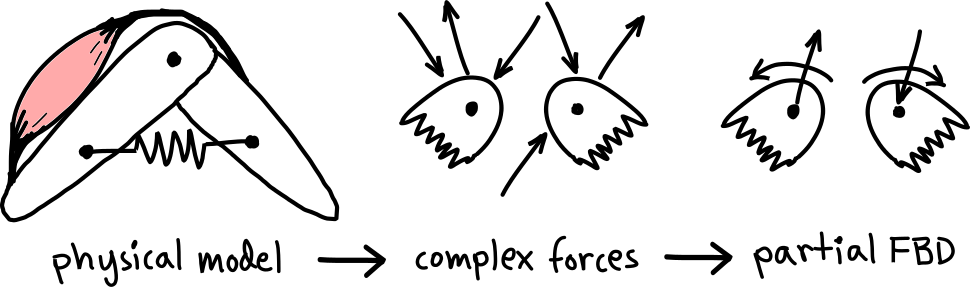
\includegraphics[width=0.8\textwidth]{Figures/ElbowFBD}\par
\end{centering}
\caption[Diagram: Free Body Diagram of an Elbow]{Free body diagram of an elbow. To analyze an animal's joint using mechanics, the physical model of the joint (including bones and muscles) is reduced to a free body diagram with a single force-couple system in at the joint.}
\label{fig:ElbowFBD}
\end{figure}
%

The muscle can be modeled as a spring that acts between two points on different bones. There are likely many forces acting on a joint, but they can be reduced to an equivalent single force and moment. The power generated at the joint is then given by the resultant moment and the angular velocity at which the joint is opening or closing.

\begin{equation}
P_{i}^{joint} = \vM \cdot \vomega_{rel}
\end{equation}

% FIGURE
\begin{figure}[h]		% h="here" t="top" b="bottom" p="separate page"
\begin{centering}
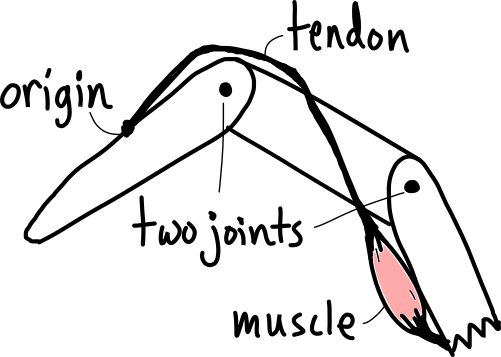
\includegraphics[width=0.3\textwidth]{Figures/TwoJoints}\par
\end{centering}
\caption[Diagram: Two-Joint Muscles]{Two-joint muscles. Some muscles act through two joints via a tendon, and accordingly the power generated by the muscle is exprssed differently than for muscles that act across only one joint.}
\label{fig:TwoJoints}
\end{figure}
%

Some muscles act through two joints, as shown in figure \ref{fig:TwoJoints}. In this case, the muscle is connected to the farther bone through a tendon. The power generated by the muscle is approximated by

\begin{equation}
P_{i}^{musc} = - T \dot{l}
\end{equation}

where $T$ is the tension in the muscle and $l$ is the length of the muscle, as in figure \ref{fig:OneMuscle}.

% FIGURE
\begin{figure}[h]		% h="here" t="top" b="bottom" p="separate page"
\begin{centering}
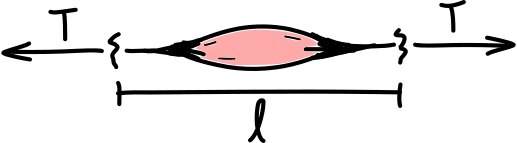
\includegraphics[width=0.4\textwidth]{Figures/OneMuscle}\par
\end{centering}
\caption[Diagram: Muscle tension]{Muscle tension. The power generated by a muscle can be expressed as the product of the tension in the muscle and the rate of its elongation.}
\label{fig:OneMuscle}
\end{figure}
%
[chris: this would be a good place to dicuss concentric and eccentric contractions]
By analyzing muscles in this way, it is possible to quantify the overall level of muscle activity occuring in a locomotive. This provides an ``inside-out'' method of calculating the power generated by the muscles of a locomotive. Logically, this ``inside-out'' method is more arduous and riddled with complexity than perhaps an outside observation of energy usage.

\section{Measuring Power}
\label{sec:MeasuringPower}
\index{measuring power}

We can deductively determine the muscle activity by finding $P^{int}$ externally, through experiments. The simplest type of experiment is having a locomotive perform a gait on a force plate, as shown in figure \ref{fig:ForcePlate}. A likely setup is to place the force plate under a tread mill on which the locomotive moves in place. The force plate then records the vertical force exerted by the locomotive $\vF^{tot}(t)$ as a function of time.

% FIGURE
\begin{figure}[h]		% h="here" t="top" b="bottom" p="separate page"
\begin{centering}
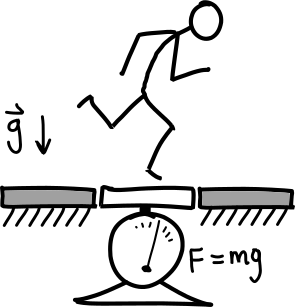
\includegraphics[width=0.25\textwidth]{Figures/ForcePlate}\par
\end{centering}
\caption[Diagram: Force Plate]{Force plate. A force plate is used to measure the force that a locomotive exerts on the ground during its locomotion. It is possible to use a force plate to estimate the power usage of a locomotive. Multiple force plates can be used (perhaps one per foot) to obtain more detailed results.}
\label{fig:ForcePlate}
\end{figure}
%

The recorded force can be divided into two parts.

\begin{equation}
\vF^{tot}(t) = \vF^{G} + mg \uj
\end{equation}

where $\vF^{G}$ is the reaction force of the ground on the locomotive. The acceleration of the center of mass $\va_{G}(t)$ is

\begin{equation}
\va_{G}(t) = \vF^{tot}/m_{tot}
\end{equation}

The velocity, which is required to find power, is determined by integrating this acceleration over time.

\begin{equation}
\vv(t) = \vv(t=0) + \int_{0}^{t} \va(\tau) d\tau
\label{eq:VelocityIntegral}
\end{equation}

Note that the force plate measures a vertical force only. As a result, the acceleration provided is a vertical acceleration. If the locomotive maintains a constant horizontal velocity, then the error from using the force plate measurement to calculate $\va(t)$ is minimal. To find the velocity at any time, the initial velocity must be known. If the motion is assumed to be periodic, then the integral of the velocity over a period of the gait divided by the period is equal to the locomotive's average velocity. Additionally, the integral of the total acceleration over a period of the gait is zero.

\begin{align}
\bar{\vv} &= \frac{1}{T}\int_{0}^{T} \vv(\tau)d\tau \notag \\
&= \frac{1}{T} \int_0^{T} \left( \vv(0) + \int_{0}^{t} \va(t') dt' \right) dt \\
0 &= \int_{0}^{T} \va(t)dt
\label{eq:VelocityIntegralAverage}
\end{align}

Equation\ref{eq:VelocityIntegralAverage} can be solved for the initial velocity, assuming that the average velocity can also be measured. The quantities $\vv_{G}$ and $\va_{G}$ can be used to calculate $\KEdot_{G}$

\begin{equation}
\KEdot_{G}(t) = m_{tot} \vv_{G}(t) \cdot \va_{G}(t)
\end{equation}

Furthermore, the measured velocity and acceleration can be related to the biomechanics power terms introduced earlier

\begin{align}
\KEdot_{G} &= (P_{bio}^{ext})^{\prime} + P_{grav} \notag \\
&= m_{tot} \vv_{G} \cdot \va_{G} + m_{tot} g \uj \cdot \vv_{G} \label{eq:ForcePlatePower} \\
\end{align}

The prime is placed equation \ref{eq:ForcePlatePower} because the gravity power has been separated out as an external force from $P_{bio}^{ext}$. This biomechanis external power can also be called the ``center of mass power''. In the context of such force plate experiments, the terms ``internal power'' and ``external power'' in the biomechanics literature refer to the biomechanics definitions of power in equations \ref{eq:PbioInt} and \ref{eq:PbioExt}. Note that the mechanics external power, $P^{ext}$, can still be approximated as zero. [chris: need clarificaiton about how a(t) is calculated; e.g. if it includes gravity force, and why Pgrav is separated from P bio ext]

A better experiment can be performed if two force plates are used rather than just one. This method, pioneered by Donelan and Kuo \cite{donelan01}, is called the \emph{individual limbs method}\index{individual limbs method}. It is posited that a single force plate does not gather enough information. Mathematical negative/positive force cancellation causes information about energy interactions during walking to be lost.

In this case, force is measured separately for the leading and trailing legs. Two power terms are found, as in equation \ref{eq:IndividualLimbs}, one for each leg. [chris: need to actually read the donelan paper].

\begin{align}
P_{lead} &= \vF_{lead} \cdot \vv_{G} \\
P_{trail} &= \vF_{trail} \cdot \vv_{G}
\label{eq:IndividualLimbs}
\end{align}
